\section{Μοντέλο Οντοτήτων/Συσχετίσεων}

\subsection{Γενική Περιγραφή}

Οι οντότητες είναι : οι Εκδήλωση, η Τοποθεσία, η Ημερομηνία, ο Καλλιτέχνης - Διοργανωτής, η Αγορά Εισιτηρίων και η Προσβασιμότητα. Για κάθε εκδήλωση θα πρέεπι να καταγράφεται το όνομά της, το είδος της και το όνομα του καλλιτέχνη-διοργανωτή.
\\
\\
\underline{Υποθέσεις:}
\begin{itemize}[noitemsep]

\item Ο κωδικός εκδήλωσης είναι μοναδικός για κάθε εκδήλωση. Για παράδειγμα, εφόσον ο κωδικός 101 αντιστοιχεί σε μια συγκικριμένη εκδήλωση (ασχέτως καλλιτέχνη ή τοποθεσίας), την ημερομηνία 1/12/2018, τότε ο ίδιος κωδικός δεν μπορεί να είναι κωδικός καμίας άλλης εκδήλωσης.
\item Οι εκδηλώσεις θα θεωρούμε ότι είναι μόνο καλλιτεχνικές και όχι με προώθηση οργανισμών ή ιδεολογιων.


\end{itemize}

\subsection{Καθορισμός Οντοτήτων}

Παρακάτω φαίνονται οι οντότητες της \titlos, η περιγραφή τους καθώς και κάποια γνωρίσματά τους.

\begin{center}
\begin{tabular}[]{|c | c|}
\hline
\textbf{Όνομα Οντότητας}   &  Event  \\ \hline 
\textbf{Περιγραφή}         &  Οντότητα που αποθηκεύονται οι εκδηλώσεις \\ \hline 
\textbf{Ιδιότητες}         &  Ισχυρή οντότητα \\  \hline               
\textbf{Γνωρίσματα}        &  \underline{Κωδικός εκδήλωσης} \\
                           &  Όνομα καλλιτέχνη\\
           ~               &  Είδος εκδήλωσης \\
            ~              &  Ύπαρξη Εισιτηρίου \\
             ~             &  Κοινό που απευθύνεται \\
              ~            &  Σκοπός \\ 
\hline
\hline
\textbf{Όνομα Οντότητας}   &  Location \\ \hline 
\textbf{Περιγραφή}         &  Οντότητα που αποθηκεύονται οι τοποθεσίες των εκδηλώσεων \\ \hline 
\textbf{Ιδιότητες}         &  Ασθενής οντότητα \\ \hline 
\textbf{Γνωρίσματα}        &  \underline{Κωδικός τοποθεσίας} \\
                           &  \underline{Κωδικός εκδήλωσης}\\
           ~               &  Εσωτερικός ή Εξωτερικός χώρος \\
            ~              &  Κατάλογος τιμών \\
             ~             &  ΤΚ (αντι για πολη περιοχη?)\\
\hline
\hline
\textbf{Όνομα Οντότητας}   &  Date \\ \hline 
\textbf{Περιγραφή}         &  Οντότητα που αποθηκεύονται οι ημερομηνίες των εκδηλώσεων \\ \hline 
\textbf{Ιδιότητες}         &  Ασθενής οντότητα \\ \hline 
\textbf{Γνωρίσματα}        &  \underline{Κωδικός εκδήλωσης}\\
                           &  \underline{Ημέρα} \\
           ~               &  Ώρα \\
            ~              &  Αναμενόμενες καιρικές συνθήκες \\
\hline
\end{tabular}

\begin{tabular}[]{|c | c | } 
\hline
\textbf{Όνομα Οντότητας}   &  Artist \\ \hline 
\textbf{Περιγραφή}         &  Οντότητα που αποθηκεύονται οι καλλιτέχνες \\ \hline 
\textbf{Ιδιότητες}         &  Ισχυρή οντότητα    \\    \hline           
\textbf{Γνωρίσματα}        &  \underline{Όνομα καλλιτέχνη}\\
           ~               &  Καταγωγή \\
            ~              &  Είδος \\
\hline 
\hline
\textbf{Όνομα Οντότητας}   &  Tickets \\ \hline 
\textbf{Περιγραφή}         &  Οντότητα που αποθηκεύονται οι τρόποι αγοράς εισιτηρίων \\\hline 
\textbf{Ιδιότητες}         &  Ασθενής οντότητα \\       \hline           
\textbf{Γνωρίσματα}        &  \underline{Κωδικός εκδήλωσης} \\
                           &  Ύπαρξη εισιτηρίου \\
                           &  Φυσικά καταστήματα προπώλησης \\
           ~               &  Ηλεκτρονικά καταστήματα προπώλησης \\
            ~              &  Εύρος τιμών \\
\hline 
\hline
\textbf{Όνομα Οντότητας}   &  Accessibility \\ \hline 
\textbf{Περιγραφή}         &  Οντότητα που αποθηκεύονται οι τρόποι πρόσβασης στην τοποθεσια \\ \hline 
\textbf{Ιδιότητες}         &  Ασθενής οντότητα \\  \hline                 
\textbf{Γνωρίσματα}        &  \underline{Κωδικός Τοποθεσίας} \\
                           &  Ύπαρξη χώρου στάθμευσης\\
            ~              &  Ύπαρξη κοντινών στάσεων \\
             ~             &  Ύπαρξη υποδομών για ΑΜΕΑ \\
                           & { \begin{tabular}[]{c|c}
                             Ύπαρξη τοποθεσιών με μισθωμένα ΜΜΜ & ναι/όχι \\
                                                                & τοποθεσία \\
                                                                & ώρα \\ 
                           \end{tabular} }  
\\ \hline
\end{tabular}
\end{center}


\subsection{Καθορισμός Συσχετίσεων}

Παρακάτω αναφέρονται οι συσχετίσεις της βάσης δεδομένων \titlos

\begin{tabular}[]{|p{4cm}|p{10cm}|}
  \hline
  \textbf{Όνομα Συσχέτισης} & Event\_Has\_Artist\\ \hline
  \textbf{Περιγραφή} & Κάθε εκδήλωση πρέπει να έχει 1 καλλιτέχνη\\ \hline
  \textbf{Ιδιότητες} & Has-A \{αναφέρετε αν είναι Is-A και αν είναι
                       Αναδρομική, Προσδιορίζουσα, Τριαδική\} \\ \hline
  \textbf{Λόγος πληθικότητας} & n:1 \\ \hline
  \textbf{Συμμετοχή} & Ολική Συμμετοχή του Event \\ \cline{2-2}
                     & Μερική Συμμετοχή του Artist \\ \hline
  \textbf{Γνωρίσματα} & - \\ \hline
\end{tabular}


\begin{tabular}[]{|p{4cm}|p{10cm}|}
  \hline
  \textbf{Όνομα Συσχέτισης} & Event\_Has\_Location\\ \hline
  \textbf{Περιγραφή} & Κάθε εκδήλωση πρέπει να έχει 1 τοποθεσία\\ \hline
  \textbf{Ιδιότητες} & Has-A \{αναφέρετε αν είναι Is-A και αν είναι
                       Αναδρομική, Προσδιορίζουσα, Τριαδική\} \\ \hline
  \textbf{Λόγος πληθικότητας} & n:1 \\ \hline
  \textbf{Συμμετοχή} & Ολική Συμμετοχή του Event \\ \cline{2-2}
                     & Μερική Συμμετοχή του Location \\ \hline
  \textbf{Γνωρίσματα} & - \\ \hline
\end{tabular}


\begin{tabular}[]{|p{4cm}|p{10cm}|}
  \hline
  \textbf{Όνομα Συσχέτισης} & Event\_Has\_Date\\ \hline
  \textbf{Περιγραφή} & Κάθε εκδήλωση πρέπει να έχει 1 ημερομηνία\\ \hline
  \textbf{Ιδιότητες} & Has-A \{αναφέρετε αν είναι Is-A και αν είναι
                       Αναδρομική, Προσδιορίζουσα, Τριαδική\} \\ \hline
  \textbf{Λόγος πληθικότητας} & n:1 \\ \hline
  \textbf{Συμμετοχή} & Ολική Συμμετοχή του Event \\ \cline{2-2}
                     & Μερική Συμμετοχή του Date \\ \hline
  \textbf{Γνωρίσματα} & - \\ \hline
\end{tabular}


\begin{tabular}[]{|p{4cm}|p{10cm}|}
  \hline
  \textbf{Όνομα Συσχέτισης} & Event\_Has\_Date\\ \hline
  \textbf{Περιγραφή} & Κάθε εκδήλωση πρέπει να έχει 1 ημερομηνία\\ \hline
  \textbf{Ιδιότητες} & Has-A \{αναφέρετε αν είναι Is-A και αν είναι
                       Αναδρομική, Προσδιορίζουσα, Τριαδική\} \\ \hline
  \textbf{Λόγος πληθικότητας} & n:1 \\ \hline
  \textbf{Συμμετοχή} & Ολική Συμμετοχή του Event \\ \cline{2-2}
                     & Μερική Συμμετοχή του Date \\ \hline
  \textbf{Γνωρίσματα} & - \\ \hline
\end{tabular}

\begin{tabular}[]{|p{4cm}|p{10cm}|}
  \hline
  \textbf{Όνομα Συσχέτισης} & Event\_Has\_Tickets\\ \hline
  \textbf{Περιγραφή} & Κάθε εκδήλωση πρέπει να έχει μέρη που πωλούνται εισιτήρια\\ \hline
  \textbf{Ιδιότητες} & Has-A \{αναφέρετε αν είναι Is-A και αν είναι
                       Αναδρομική, Προσδιορίζουσα, Τριαδική\} \\ \hline
  \textbf{Λόγος πληθικότητας} & n:1 \\ \hline
  \textbf{Συμμετοχή} & Ολική Συμμετοχή του Event \\ \cline{2-2}
                     & Μερική Συμμετοχή του Tickets\\ \hline
  \textbf{Γνωρίσματα} & - \\ \hline
\end{tabular}

\begin{tabular}[]{|p{4cm}|p{10cm}|}
  \hline
  \textbf{Όνομα Συσχέτισης} & Location\_Has\_Accessibility\\ \hline
  \textbf{Περιγραφή} & Κάθε τοποθεσία πρέπει να έχει τρόπους πρόσβασης\\ \hline
  \textbf{Ιδιότητες} & Has-A \{αναφέρετε αν είναι Is-A και αν είναι
                       Αναδρομική, Προσδιορίζουσα, Τριαδική\} \\ \hline
  \textbf{Λόγος πληθικότητας} & n:1 \\ \hline
  \textbf{Συμμετοχή} & Ολική Συμμετοχή του Location \\ \cline{2-2}
                     & Μερική Συμμετοχή του Accessibility\\ \hline
  \textbf{Γνωρίσματα} & - \\ \hline
\end{tabular}

\subsection{Διάγραμμα Οντοτήτων/Συσχετίσεων}

\{Δείξτε το διάγραμμα Ο/Σ για τη βάση. Το διάγραμμα μπορείτε να το
κατασκευάσετε σε πρόγραμμα της επιλογής σας, ωστόσο θα πρέπει να
ακολουθεί το συμβολισμό Chen (δηλαδή οντότητες ως παραλληλόγραμμα,
συσχετίσεις ως ρόμβοι, διπλή γραμμή για υποχρεωτική συμμετοχή, κτλ.)\}

Παράδειγμα για τη FlightsDB:
\begin{figure}[H]
  \centering
  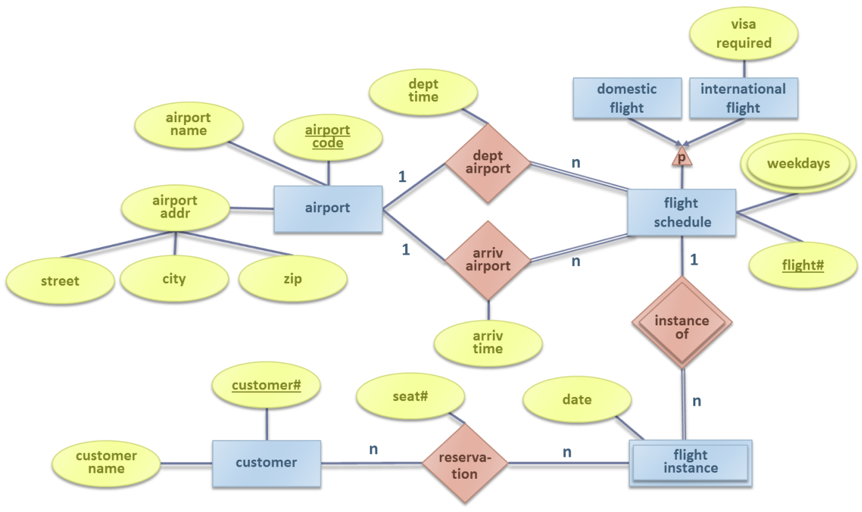
\includegraphics[width=\linewidth]{entities.png}
  \caption{Διάγραμμα Οντοτήτων/Συσχετίσεων}
\end{figure}


%%% Local Variables:
%%% mode: latex
%%% TeX-master: "main"
%%% End:
